\subsection{Calculos circuito simple en dispociosición triangulo para haz de un solo conductor}

\begin{figure}[ht!]
    \centering
    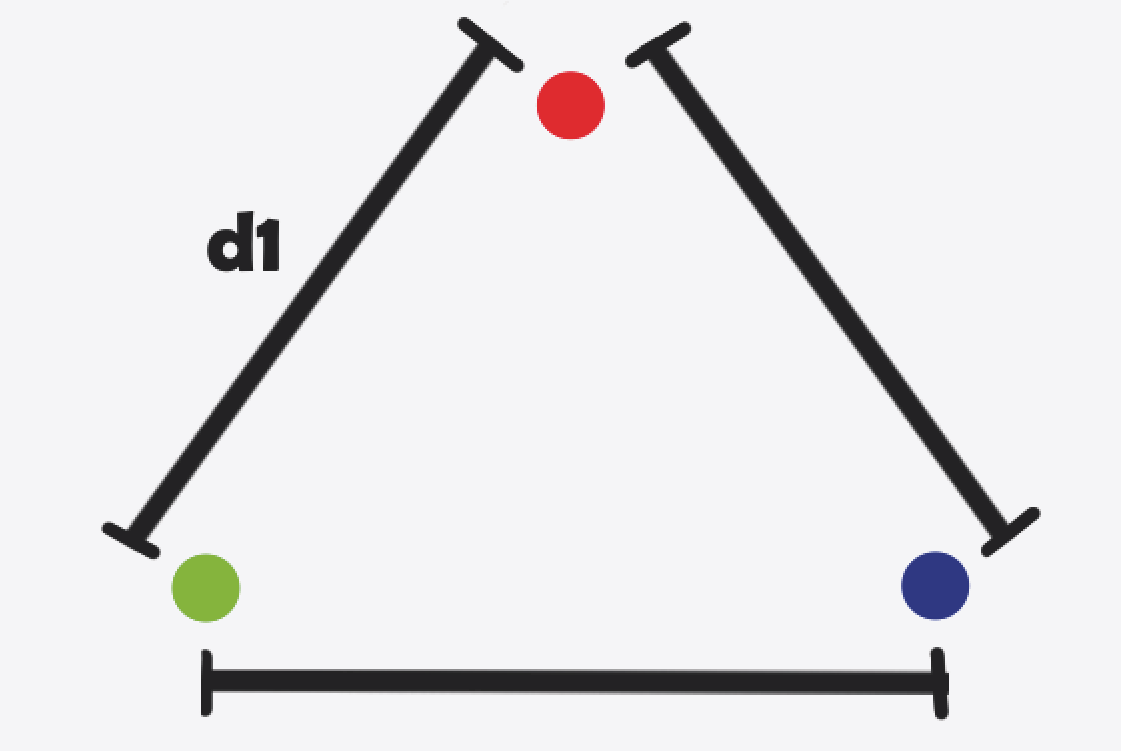
\includegraphics[width=0.48\textwidth]{img/Calculos circuito simple en dispociosición triangulo para haz de un solo conductor disp.png}
    \caption{circuito simple con fases en dispociosición triangulo para haz de un solo conductor.}
    \label{fig:circuito_simple_disp}
\end{figure}

\begin{figure}[ht!]
    \centering
    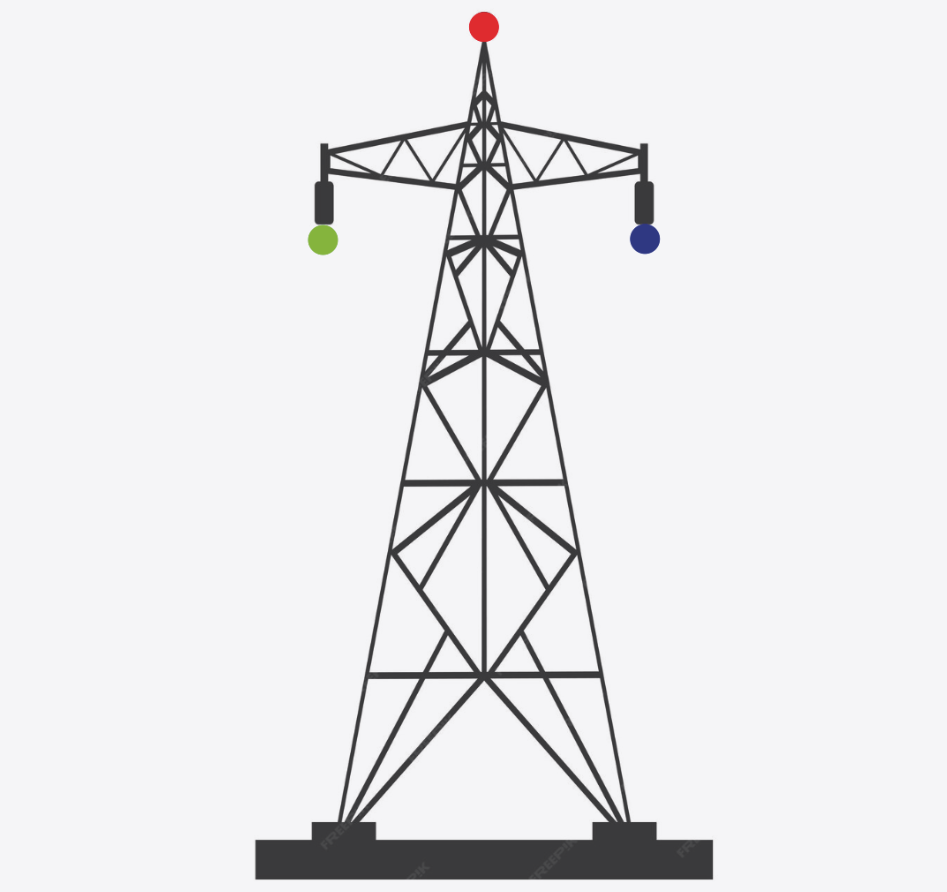
\includegraphics[width=0.48\textwidth]{img/Calculos circuito simple en dispociosición triangulo para haz de un solo conductor.png}
    \caption{circuito simple con fases en dispociosición triangulo para haz de un solo conductor.}
    \label{fig:circuito_simple_Torre}
\end{figure}



\textbf{Datos del conductor: Flint 746,4 kcmil}
\begin{itemize}
  \item Longitud línea: $l = 31 \, \text{km}$
  \item Temperatura: $T = 28^\circ$C
  \item $s = 0.4572$ [m]
  \item Radio: $r = 12.58$ [mm]
  \item $f = 60$ [Hz]
  \item RMG = 9.66 [cm]
  \item Resistencia a 75°C: $R_{75} = 0.106 \, \Omega/\text{km}$
  \item $\alpha_0$ aluminio = 0.00438
\end{itemize}

\vspace{0.5cm}

\subsection*{Cálculo de Resistencia equivalente por fase:}

\[
R_{28} = \left( \frac{1 + \alpha_0 \cdot28}{1 + \alpha_0 \cdot 75} \right) \cdot R_{75} = 0.0895488 \, \frac{\Omega}{\text{km}}
\]

\[
R_{\text{eq}} = 0.0895488 \, \frac{\Omega}{\text{km}} = 0.0895488 \cdot 31 = 2.7768 \, [\Omega]
\]

\vspace{0.5cm}
\subsection*{Cálculo de Reactancia Inductiva:}


\[
DMG_{e} = \sqrt[3]{d1 \cdot d1 \cdot d1} = 12 \, [\text{m}]
\]

\vspace{0.3cm}
\[
RMG_{e} = radio\cdot e^{(-1/4)} = 9.7973 \, [\text{mm}]
\]

\vspace{0.3cm}
\[
X_L = 31\cdot 2\pi \cdot f \cdot2\cdot 10^{-4} \cdot \ln\left( \frac{DM_{Ge}}{RMG_e} \right) = 16.6198\, [\Omega]
\]

\[
z_T = \left[ R_{\text{eq}T} + jX_L \right] = 2.7768 + j16.6198 \quad [\Omega]
\]

\subsection*{Cálculo de la capacitancia:}

\[
RMG_{e} = radio = 12.58 \, [\text{mm}]
\]

\[
C_T = \left[ 31 \cdot \left(18 \cdot 10^9 \cdot \ln\left( \frac{DMG_e}{RMG_e} \right) \right)^{-1} \right]
\]

\[
C_T =  242.2065 \, [nF]
\]


\[
Y_T = j\cdot2\pi \cdot f \cdot C_T = j91.309 \, [\mu S]
\]

\section*{Parámetros de la línea y receptor:}

\begin{align*}
A &= 1 + \frac{Z_T \cdot Y_T}{2} = 0.9992 + j\,1.2677 \times 10^{-4} \\
B &= Z_T = 2.7768 +16.6198i \quad [\Omega] \\
C &= Y_T \left(1 + \frac{Z_T \cdot Y_T}{4} \right) \\
C &= C = -5.7879e-09 + 9.1275e-05i \quad [S] \\
D &= A =  0.9992 + j\,1.2677 \times 10^{-4} 
\end{align*}

\begin{align*}
I_R &= \frac{S}{\sqrt{3} \cdot V_L} \cdot \angle -\cos(\text{fp})  \\
I_R &= 1757.15299 \angle  -25.84193 ^\circ \quad [A] \\
V_R &= \frac{V_L}{\sqrt{3}} \angle 0^\circ = 132.79056 \angle 0^\circ \quad [kV]
\end{align*}

\section*{Parámetros del Generador}

\begin{align*}
V_G &= A \cdot V_R + B \cdot I_R \\
I_G &= B \cdot V_R + D \cdot I_R
\end{align*}

\begin{align*}
V_G &= 151.7484 \angle 9.16614^\circ \quad [kV] \\
I_G &= 1750.5712 \angle -25.477^\circ \quad [A]
\end{align*}

\[
\%RV = \left( \frac{ |V_G| }{ |A| \cdot |V_R| } \right) - 1 = 14.3633\%
\]
\[
\% \text{Pérdida} = 100*\frac{P_g - P_r}{P_g} =  3.9113\%
\]
\[
\% \eta =100* \frac{P_r}{P_g} = 96.0887\%
\]

\section*{Efecto Corona}

\begin{align*}
m_c &= 0{,}95 \\
m_t &= 1 \\
r &= 400 \quad [\text{m}] \\
T &= 28^\circ \text{C}
\end{align*}

\begin{align*}
h &= 10^{\log_{10}(76) - \frac{y}{18336}} \Rightarrow h = 72.2767 \\
\delta &= \frac{3{,}921 \cdot h}{273 + T} = 0.9410
\end{align*}

\begin{align*}
U_c &= 84 \cdot m_c \cdot m_t \cdot \delta \cdot \log \left( \frac{DMG}{r} \right) \quad [\text{kV}]
\end{align*}

\begin{align*}
U_{ne} &= 1{,}15 \cdot U_{\text{línea}} \quad [\text{kV}]
\end{align*}

\begin{align*}
U_{ne} < U_c &\Rightarrow 264.5 \leq 281.4748 \\
&\text{No se presenta efecto Corona}
\end{align*}